\textbf{\textit{Soal. }}Diberikan segitiga $ABC$ dengan besar sudut $\angle ABC = 60^\circ$ dan $\angle BCA = 100^\circ$. Pada sisi $AB$ dan $AC$ berturut-turut terdapat titik $D$ dan $E$ sehingga $\angle EDC = 2\angle BCD = 2\angle CAB$. Tentukan besar sudut $\angle BED$.
\begin{proof}[\textbf{Solusi. }] (Tuesday, 19 September 2023) Diketahuhi $\angle CAB = 180^\circ - 60^\circ - 100^\circ = 20^\circ$. Oleh karena itu jelas bahwa $\angle EDC = 2\angle CAB = 40^\circ$ dan $\angle BCD = \angle CAB = 20^\circ$. Selain itu $\angle DCA = \angle BCA - \angle BCD = 80^\circ$ sehingga $\angle CDA = 180^\circ - \angle DAC - \angle DCA = 80^\circ$ yang menyebabkan $DA=AC$ dan $\angle CDE = \angle EDA = 40^\circ$.
    % \begin{center}
    \begin{asy}
        import olympiad;
        import geometry;
        size(300);
        pair B = (0,0);
        pair C = (1,-3);
        pair A = (8.92055, -1.82546);
        pair D = (1.07595, -0.22018);
        pair E = (3.0417, -2.69723);
        dot("$A$", A, NE);
        dot("$B$", B, SW);
        dot("$C$", C, SW);
        dot("$D$", D, N);
        dot("$E$", E, S);
        draw(A--B--C--A);
        draw(C--D--E--B, red);
    \end{asy}
\end{center}
    \begin{center}
    \begin{tikzpicture}[scale=0.8, dot/.style={circle, fill, inner sep=0.5pt, outer sep=0pt}]

        \tkzDefPoint(0,0){B}
        \tkzDefPoint(1,-3){C}
        \tkzDefPoint(8.92055,-1.82546){A}
        \tkzDefPoint(1.07595,-0.22018){D}
        \tkzDefPoint(3.0417,-2.69723){E}

        \tkzDrawPolygon(A,B,C)
        \tkzDrawSegments[red](C,D D,E E,B)

        \tkzDrawPoints[fill=black, size=3](A,B,C,D,E)
        \tkzLabelPoint[above right](A){$A$}
        \tkzLabelPoint[below left](B){$B$}
        \tkzLabelPoint[below left](C){$C$}
        \tkzLabelPoint[above](D){$D$}
        \tkzLabelPoint[below](E){$E$}

    \end{tikzpicture}
\end{center}

Dari fakta tersebut, dengan Angle Bisector Theorem berlaku $\dfrac{CD}{DA} = \dfrac{CE}{EA}$.
Selain itu, karena $\angle DBC = \angle CBA$ dan $\angle BAC = \angle BCD$ maka $\triangle BDC \sim \triangle BCA$ sehingga $\dfrac{BC}{AB} = \dfrac{BD}{CB} = \dfrac{CD}{CA}$.

\begin{lemmarev}
    $BE$ garis bagi $\angle CBA$
    \begin{proof}
        \textbf{Alternatif 1.}\\
        Oleh karena itu, dengan menggabungkan fakta-fakta sebelumnya dan dengan dalil sinus pada $\triangle CDA$ dan $\triangle BDC$ kita punya
        \begin{align*}
            \dfrac{BC}{AB}=\dfrac{BD}{CB} = \dfrac{\sin 20^\circ}{\sin 100^\circ} = \dfrac{\sin 20^\circ}{\sin 80^\circ} = \dfrac{CD}{DA} = \dfrac{CE}{EA}
        \end{align*}
        \textbf{Alternatif 2.}\\
        Kita punya
        \begin{align*}
            \dfrac{CE}{EA} = \dfrac{CD}{AD} = \dfrac{CD}{AC}  = \dfrac{BC}{AB}
        \end{align*}
        sehingga dari alternatif 1 atau alternatif 2 tersebut, berdasarkan Angle Bisector Theorem menunjukkan bahwa $BE$ adalah garis bagi $\angle CBA$.
    \end{proof}
\end{lemmarev}
Dari sini, $\angle EBD = \frac{1}{2}\angle CBA = 30^\circ$ sehingga $\angle DEB = 180^\circ - \angle EBD - \angle BDE = 180^\circ - 30^\circ - (100^\circ + 40^\circ) = 10^\circ$.
\end{proof}